\documentclass[times, utf8, diplomski]{fer}
\usepackage{booktabs}
\usepackage[utf8]{inputenc}

\usepackage[T1]{fontenc}
\usepackage{fixltx2e}
\usepackage{graphicx}
\usepackage{longtable}
\usepackage{float}
\usepackage{wrapfig}
\usepackage{soul}
\usepackage{textcomp}
\usepackage{marvosym}
\usepackage{wasysym}
\usepackage{latexsym}
\usepackage{amssymb}
\usepackage{hyperref}
\usepackage{caption}
\usepackage{pdfpages}
\usepackage{float}
%\usepackage[usenames, dvipsnames]{color}
\usepackage{listings}
\usepackage{xcolor}
\usepackage{subfig}
\usepackage{algpseudocode}
\usepackage[Algoritam]{algorithm}
\usepackage{amssymb}

\lstset { %
    language=C++,
    backgroundcolor=\color{black!5}, % set backgroundcolor
    basicstyle=\footnotesize,% basic font setting
}


\begin{document}

\thesisnumber{570}

\title{Tool for aligning long DNA reads}

\author{Filip Paveti\'{c}}

\maketitle

% Ispis stranice s napomenom o umetanju izvornika rada. Uklonite naredbu \izvornik ako želite izbaciti tu stranicu.
\izvornik

% Dodavanje zahvale ili prazne stranice. Ako ne želite dodati zahvalu, naredbu ostavite radi prazne stranice.
\zahvala{}

\tableofcontents

\chapter{Introduction}
Uvod rada. Nakon uvoda dolaze poglavlja u kojima se obrađuje tema.

\chapter{Preliminaries}

From algorithmic point of view, aligning reads to a reference genome comes down to string pattern matching. When looked that way, one does not have to know a lot of biology background in order to understand how the existing alignment systems work. However, to understand a wider picture it is useful to know some basic genetics. 
\\
\\
This chapter is intended to give a short introduction to genetics. There exist many resources which cover this topic in far more depth\cite{griffiths}\cite{brown}. Additionaly, terminology used through rest of the Thesis is introduced. In the end of the chapter, basic alignment algorithms are discussed in details.

\section{Genetics}
\subsection{Overview}

\emph{Genetics} is a field of science which studies \emph{genes}. Genes are the carrier of biological information in the living organisms. They are responsible for inheritance of features from organisms to their offsprings. Aside from carrying that hereditary information, the role of genes inside a cell of an organism is to dictate production of molecules called \emph{proteins}. If we think of a gene as a part of the cell which commands what to do, protein is the part which does the job. Each type of protein is specialized for a particular job, such as catalyzing metabolic reactions, replicating  DNA or transporting molecules from one place to another.
\\
\\
Protein is structured as a chain of twenty different kinds of molecules called \emph{amino-acids}. Interaction between those molecules causes the protein to fold into a compact shape (Figure \ref{myoglobin}). Shape and sequence of amino-acids determine what a protein does. For example, protein can match the shape of another molecule, which would allow the protein to bind around that molecule and transport it.

\begin{figure}[!ht]
\begin{center}
	\includegraphics[width=0.7\textwidth]{../img/Myoglobin.png}
	\caption{3D structure of Myoglobin protein (http://en.wikipedia.org/wiki/Myoglobin, June 11th 2013)}\label{myoglobin}
\end{center}
\end{figure}

\subsection{From genes to proteins}

\emph{DNA (deoxyribonucleid acid)} is a long molecule which encodes genetic instructions in living organisms. That molecule consists of two interconnected chains (\emph{strands}) which are consisted of alternating sugar and phosphate groups with one of four kind of \emph{nucleobases} attached to the sugars. Nucleobases found in the DNA are: guanine, adenine, thymine and cytosine encoded using letters G, A, T and C respectively. Bases on the two strands are always paired: next to adenine on one strand there is always thymine on the other. Next to guanine there is always cytosine. Due to their chemical composition, strands have directionality. Ends of strands are denoted by 5' and 3'. Those numbers refer to the orientation of fifth and third carbon atom sugar molecules are facing. Many processes involving DNA are directed (for example, replication occurs only in 5'-3' direction). Total DNA of an organism is packed inside of one or more structures called \emph{chromosomes}. Genes are only special segments of DNA which encode instruction for protein production. Set of all genes in an organism is called the \emph{genome}.
\\

\begin{figure}[!ht]
\begin{center}
	\includegraphics[width=0.5\textwidth]{../img/DNA_chemical_structure.pdf}
	\caption{DNA chemical structure (http://en.wikipedia.org/wiki/Genes, June 11th 2013), Madeleine Price Ball}\label{dna.chemical.structure}
\end{center}
\end{figure}

Process of protein production contains several steps. First, cell reads a gene and \emph{transcribes} it into \emph{RNA} chain. That molecule either has a function on its own or is passed to a structure called \emph{ribosome} - its role is to \emph{translate} received RNA to a protein.
\\

\begin{figure}[!ht]
\begin{center}
	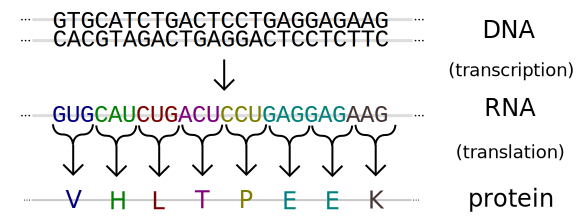
\includegraphics[width=0.7\textwidth]{../img/Genetic_code.pdf}
	\caption{DNA chemical structure (http://en.wikipedia.org/wiki/Introduction\_to\_genetics, June 11th 2013), Madeleine Price Ball}\label{genetic.code}
\end{center}
\end{figure}

Transcription step is conceptually straight forward - one of the strands of DNA is copied replacing every thymine (T) occurence with uracil (U), creating the RNA chain. Finally in the translation step RNA is passed to a ribosome. It translates consecutive triplets of bases into corresponding amino-acids resulting in a protein. 

\section{Shotgun DNA sequencing}

Shotgun sequencing is a method of determining the order of nucleotides in long DNA strands. Current technologies allow efficients sequencing of fairly short strands (100 to 1000 basepairs). That is why a long strand is copied several times and each clone broken at random places into \emph{fragments}. This process inspired the name of the method since it imitates random firing pattern of an actual shotgun. Due to loss of precision not entire fragments are actually read. In the case of \emph{single} end sequencing some number of bases from one end of the fragment is read whereas in the case of \emph{paired} end sequencing both ends are read simultaneously, keeping track of distance between them and their orientation. After DNA reads of an organism have been accumulated\footnote{One accepted way is to produce one or two files in the FASTQ format, depending on whether it is a single or paired end sequencing involved.}, DNA is then assembled with the help of computers. 

\begin{figure}[!ht]
\begin{center}
	\includegraphics[width=0.85\textwidth]{../img/Whole_genome_shotgun_sequencing.png}
	\caption{Whole genome shotgun sequencing}\label{shotgun.sequencing}
\end{center}
\end{figure}

\section{Alignment algorithms}

One of the fundamental problems of finding good overlap between reads or aligning them to a reference genome is that the matchings we are looking for need not to be perfect. This is a consequence of errors which are introduced to the reads, either by the sequencing process or by mutations. In order to deal with that, algorithms such as Smith-Waterman, Needleman-Wunsch and Levenshtein distance have been developed (TODO: referencirati). In the succeeding section algorithm for calculating the Levenshtein distance is described. The section will introduce the basic concept on top of the other mentioned algorithms are built as well.

\subsection{Edit (Levenshtein) distance}

Levenshtein or edit distance is a metric measuring the difference between two sequences. Simply stated, it is a minimum number of single character edits (insertions, deletions and substitutions) required to change one word into the other.
\\
\\
Mathematically, edit distance of strings $a$ and $b$ is given by $d_{a,b}(|a|,|b|)$ where:

\begin{eqnarray}
	\label{levenshtein}
	d_{a,b}\left(i,j\right) & = & 
							\left\{
								\begin{array}{ll}
								max(i,j) & \mbox{if } min(i,j) = 0\\	
								min\left\{
									\begin{array}{ll}
									d_{a,b}(i-1,j)\\	
									d_{a,b}(i,j-1)\\	
									d_{a,b}(i-1,j-1) + [a_i\ne b_i]\\	
									\end{array}
									\right.&\mbox{otherwise}\\
								\end{array}
							\right.
\end{eqnarray}

\subsubsection{Example}
Levenhstein distance between words "kitten" and "sitting" is 3, with the following sequence of operations:

\begin{enumerate}\itemsep0pt
\item \textbf{k}itten $\rightarrow$ \textbf{s}itten (substitution)
\item sitt\textbf{e}n $\rightarrow$ sitt\textbf{i}n (substitution)
\item sittin $\rightarrow$ sittin\textbf{g} (insertion)
\end{enumerate}
The simplest way to do the calculation is to fill out a table like this:

\begin{table}[H]
\centering
\small
\begin{tabular}{|c|c|c|c|c|c|c|c|}
\hline
	   &   & \textbf{k} & \textbf{i} & \textbf{t} & \textbf{t} & \textbf{e} & \textbf{n}\\
\hline
	   & 0 & 1 & 2 & 3 & 4 & 5 & 6\\
\hline
	 \textbf{s} & 1 & 1 & 2 & 3 & 4 & 5 & 6\\
\hline
	 \textbf{i} & 2 & 2 & 1 & 2 & 3 & 4 & 5\\
\hline
	 \textbf{t} & 3 & 3 & 2 & 1 & 2 & 3 & 4\\
\hline
	 \textbf{t} & 4 & 4 & 3 & 2 & 1 & 2 & 3\\
\hline
	 \textbf{i} & 5 & 5 & 4 & 3 & 2 & 2 & 3\\
\hline
	 \textbf{n} & 6 & 6 & 5 & 4 & 3 & 3 & 2\\
\hline
	 \textbf{g} & 7 & 7 & 6 & 5 & 4 & 4 & 3\\
\hline

\end{tabular}
\caption{Calculating Levenshtein distance between "kitten" and "sitting"}\label{levenshtein.table}
\end{table}

\subsubsection{Complexity}
Direct implementation of the above calculation is proportional with lengths of both input string. More precisely, there are $O(|a||b|)$ operations needed (and the same ammount of memory). If assumption that a distance between $a$ and $b$ does not exceed $k$ is fullfilled, it is enough only to fill diagonal stripe of width $2k+1$ in the matrix. Using that observation complexity is reduced to $O(k*min(|a|,|b|))$. In practice, this implementation is shown to be very usefull (for example, SNAP (TODO: citiraj)


\chapter{LISA - Longest Increasing Subsequence Aligner}
\section{Overview}
This chapter begins by an overview of the algorithms used by modern mappers. After that, approach developed in this Thesis is described in details and performance is compared with several other existing mappers.\\
\\
One of the first algorithms developed for aligning reads is a \emph{local alignment} algorithm called Smith-Waterman (TODO: citirati). Alignments received by that algorithm are considered very accurate. Unfortunately, its time-complexity\footnote{This is briefly discussed in chapter 2.} limits the usage practicality so more advanced algorithms have been developed through the years.\\
\\
Many modern mappers (such as SNAP(TODO:citirati) and SeqAlto(TODO:citirati)) are following the \emph{seed-and-extend} approach. First an index is made. Index is a structure which maps every sequence of consecutive $k$ characters (\emph{kmer}) to its positions in the reference genome. The number of different kmers in the genome is $4^k$. That is a practical observation since for $k \le 32$ kmers can be encoded in a 64-bit integer. Building the index is usually one-time procedure. It is saved on the disc and reused when processing the reads. Reads are processed in the following manner: for every kmer of a read positions are fetched from the index. Gathered positions are in fact candidate positions around which read could be placed inside the DNA. Detailed examination is made by using some of the existing alignment algorithms. As an example, SNAP uses edit-distance, whereas SeqAlto uses Needleman-Wunsch. One more thing worth noting is that index can have various implementations - SNAP implements a hash table, SeqAlto uses binary search on a sorted array.\\
\\
Existing mappers perform well when the length of the reads and sequencing error rate are small. When we increase any of those things, problems begin. The main reason for low time efficiency on longer and less accurate reads is that algorithms such as edit-distance and Needleman-Wunsch have time complexities proportional both to length of the input and the error inside it. Hence, increasing any of them requires more computing.\\
\\
LISA\footnote{Longest Increasing Subsequence Aligner} is a mapper built on the following hypothesis - TODO: hipoteza. Index is built by the SeqAlto model. This results in an time efficient and precise algorithms for read alignment, specially since the lengths of reads are increasing.

\section{Index}
\section{Alignment algorithm}
Basic intuition for the developed algorithms comes from the fact that alignments which look 'good' when observed by bare eye should have a big overlaping part, as described by (TODO: slika).\\
\\
For longer reads (length greater or equal to 500), this approach practically doesn't miss when determining the region of the genome where a read belongs. If an actual alignment is needed, parts of the reads between 'matching' regions can be aligned with one of previously mentioned alignment algorithms (e.g. edit-distance).

\subsection{Single alignment}
Ovdje opisati lis i coverge, to ce biti najzeznutiji dio
\subsection{Multiple alignment}
In the previous section aligning sequences of similar lengths is described. Since the genome can be much larger than a read, direct application of LIS and COVERAGE algorithms would give poor performance. That is why a trick is used. Entire genome is divided into blocks of length closer to the read length.
\section{Implementation}
\section{Installation}
\section{Usage}

\chapter{Results}
\section{Overview}
This section gives time performance and accuracy analysis of LISA. From genomes of several species (precisely: \emph{Yersinia Pestis}, banana and a chicken), sets of single end reads are created using the \emph{wgsim} read simulator. Time needed for solving sets and performance are compared with BWA-SW, BWA-MEM \cite{Li:2010:FAL:1741823.1741825}, SNAP and SeqAlto.\\
\\
Every test set consists of 100000 single end reads created using a \emph{wgsim} read simulator. That tool is used as it is widely accepted as a benchmarking tool. All its parameters are set to default, except for the \emph{base error rate} which is set to 0.02, 0.05 and 0.10 in three separate trials.\\
\\
Conducted trials were made on a computer with 192Gb of RAM and 12 core Intel(R) Xeon(R) CPU E5645 @ 2.40 GHz.

\section{Yersinia Pestis}
\section{Banana}
\section{Chicken}

\chapter{Conclusion}
Zaključak.

\chapter{Appendix}
\section{Fenwick tree}

\bibliography{literatura}
\bibliographystyle{plain}

\begin{sazetak}
Sažetak na hrvatskom jeziku.

\kljucnerijeci{Ključne riječi, odvojene zarezima.}
\end{sazetak}

% TODO: Navedite naslov na engleskom jeziku.
\engtitle{Title}
\begin{abstract}
Abstract.

\keywords{Keywords.}
\end{abstract}

\end{document}
